% !TeX root = Body.tex
\chapter{Results}\label{chap:Res}

In this chapter, we first show in Sec.~\ref{sec:NEMCs} our numerical results of the frictional force density $f(L_{z}, T)$, the bulk energy density $\epsilon(L_{z}, T)$ and their temperature derivatives. We also show in Sec.~\ref{sec:convcheck} that the numerical infinite-size limit $L_{x}\to\infty$ converges with $L_{z}$ and $T$ fixed.

The range of parameters in our simulation is as follows. We computed the value of $f(L_{z}, T)$ for temperatures $k_{\rm B}T/J\in\{0.0,0.1,0.2,\dots,1.9,2.0,2.02,2.04,\dots,2.48,2.50,2.6,2.7,\dots,5.0\}$ and sizes $L_{z}\in\{4,8,16,32,64\}$ with the anti-parallel and the parallel boundary conditions. For the anti-parallel boundary conditions, we set the initial state to the domain-wall state, where spin variables $\sigma_{i}$ in the upper half of the system have the same value as the spins on the upper boundary and those in the lower half as the spins on the lower boundary. For the parallel boundary conditions we set the initial state to the magnetized state, where all spin variables $\sigma_{i}$ have the same value as both of boundaries. The reason why we used these initial states is that they are the most natural ground states which correpond to each set of boundary conditions.

All the simulations are performed by the single-flip algorithm with the Metropolis rate at the temperature $T$. To obtain the observables in the non-equilibrium stationary state, we performed the equilibration process for $5000$ sweeps without shift operations and the stationarization process for $5000$ sweeps for all given parameters. We checked the convergence of the observables to the equilibrium values and the stationary values for these time regions by fitting the observables by the function $A(t)=A_{0} + A_{1}\mathrm{e}^{-t/\tau}$. The duration of $5000$ sweeps is substantially longer than the fitting parameter $\tau$, which we call the \textit{non-equilibrium relaxation time}. We performed these simulations for $480$ samples for all parameters and averaged them, and then averaged along the time direction. The statistical errors of the data presented in the present chapter are all smaller than the point size.

\section{Observed Quantities}\label{sec:NEMCs}

\subsection{Frictional Force Density $f(L_{z}, T)$}

We show the behavior of the frictional force density $f(L_{z}, T)$ in Fig.~\ref{fig:fricDens_Allsize}. For both boundary conditions, $f(L_{z}, T)$ reaches the results in Ref.~\cite{Kadau2008} with the size $L_{z}=64$. We thereby decide that the size $L_{z}=64$ is a good approximation for the limit of $L_{z}\to\infty$. Towards this limit, $f(L_{z}, T)$ increases for the anti-parallel boundary conditions, whereas $f(L_{z}, T)$ decreases for the parallel boundary. 

When the size $L_{z}$ is larger than the correlation length $\xi_{z}(\beta)$ along the $z$ direction perpendicular to the cut, the system behaves as a two-dimensional one and the effects of the boundary conditions vanish, whereas when the size $L_{z}$ is smaller than $\xi_{z}(\beta)$ the system is effectively one-dimensional. We can consider this behavior as a dimensional crossover. 

\begin{figure}[htbp]
	\centering
	\subcaptionbox{\label{fig:fricDens_Allsize_AP}}[0.90\linewidth]{\includegraphics[width=0.80\linewidth]{../../NumCalc/ClassicalSpinMC/fricDensP_Allsize_AP_.eps}}
	
	\subcaptionbox{\label{fig:fricDens_Allsize_P}}[0.90\linewidth]{\includegraphics[width=0.80\linewidth]{../../NumCalc/ClassicalSpinMC/fricDensP_Allsize_P_.eps}}
	
	\caption{Temperature dependence of $f(L_{z}, T)$ with each boundary condition: (\subref{fig:fricDens_Allsize_AP}) The anti-parallel boundary conditions; (\subref{fig:fricDens_Allsize_P}) The parallel boundary conditions.}
	\label{fig:fricDens_Allsize}
\end{figure}


%Remarkably peaks $\{T_{\rm peak}(L_{z})\}$ for both boundaries hit the temperature higher than the ordinary critical point $T_{\rm c}=2/\log\left[1+\sqrt{2}\right]$. This implies that both the ordinary phase transition and the non-equilibrium phase transition occur at two different temperatures.

\subsection{Bulk Energy Density $\epsilon(L_{z}, T)$}

We show the behavior of the bulk energy density $\epsilon(L_{z}, T)$ in Fig.~\ref{fig:EnDens_Allsize}. As the frictional force density $f(L_{z}, T)$, the bulk energy density $\epsilon(L_{z}, T)$ also indicates asymptotic behavior in the limit of $L_{z}\to\infty$ as well as difference due to the boundary conditions for small $L_{z}$, reflecting the dimensional crossover.

\begin{figure}[htbp]
	\centering
	\subcaptionbox{\label{fig:EnDens_Allsize_AP}}[0.90\linewidth]{\includegraphics[width=0.80\linewidth]{../../NumCalc/ClassicalSpinMC/EnDens_Allsize_AP_.eps}}
	
	\subcaptionbox{\label{fig:EnDens_Allsize_P}}[0.90\linewidth]{\includegraphics[width=0.80\linewidth]{../../NumCalc/ClassicalSpinMC/EnDens_Allsize_P_.eps}}
	
	\caption{Temperature dependences of $\epsilon(L_{z}, T)$ with each boundary condition: (\subref{fig:fricDens_Allsize_AP}) The anti-parallel boundary conditions; (\subref{fig:fricDens_Allsize_P}) The parallel boundary conditions.}
	\label{fig:EnDens_Allsize}
\end{figure}


\subsection{Temperature Derivatives $\partial f(L_{z}, T)/\partial T$ and $c(L_{z}, T)$}

We additionally show the behavior of temperature derivatives $\partial f(L_{z}, T)/\partial T$ and $c(L_{z},T)=\partial \epsilon(L_{z}, T)/\partial T$ in Figs.~\ref{fig:dFricDens_Allsize} and \ref{fig:dEnDens_Allsize}, respectively. They exhibit sharp peaks at a characteristic temperature $k_{\rm B}T/J=2.40$ (see the red vertical line in Fig.~\ref{fig:dFricDens_Allsize}) and $k_{\rm B}T/J=2.27$ (see the black vertical line in Fig.~\ref{fig:dEnDens_Allsize}), respectively, for both boundary conditions for the largest size $L_{z}=64$. This implies that they diverge in the limit of $L_{z}\to\infty$. We observe that the finite-size peak $k_{\rm B}T_{\rm peak}(L_{z})/J$ shifts to lower temperatures for the anti-parallel boundary conditions and to higher temperatures for the parallel boundary conditions. This observation shows us that the anti-parallel boundary conditions generate a \textit{disordering} effect, while the parallel boundary conditions generate an \textit{ordering} effect. These effects are most enhanced for small $L_{z}$.

\begin{figure}[htbp]
	\centering
	\subcaptionbox{\label{fig:dFricDens_Allsize_AP}}[0.90\linewidth]{\includegraphics[width=0.80\linewidth]{../../NumCalc/ClassicalSpinMC/dFricDensP_Allsize_AP_Bar.eps}}
	
	\subcaptionbox{\label{fig:dFricDens_Allsize_P}}[0.90\linewidth]{\includegraphics[width=0.80\linewidth]{../../NumCalc/ClassicalSpinMC/dFricDensP_Allsize_P_Bar.eps}}
	
	\caption{Temperature dependence of $\partial f(L_{z}, T)/\partial T$ with each boundary condition: (\subref{fig:dFricDens_Allsize_AP}) The anti-parallel boundary conditions; (\subref{fig:dFricDens_Allsize_P}) The parallel boundary conditions. The vertical red line in each panel indicates the non-equilibrium critical temperature $T^{\rm M}_{\rm c}(10)\simeq 2.40$, where we choose the unit $k_{\rm B}/J=1$, in the phase diagram of the two-dimensional non-equilibrium Ising model obtained in Ref.~\cite{Hucht2009b}; see Fig.~\ref{fig:NEPTinIsing_}.}
	\label{fig:dFricDens_Allsize}
\end{figure}

\begin{figure}[htbp]
	\centering
	\subcaptionbox{\label{fig:dEnDens_Allsize_AP}}[0.90\linewidth]{\includegraphics[width=0.80\linewidth]{../../NumCalc/ClassicalSpinMC/dEnDens_Allsize_AP_Bar.eps}}
	
	\subcaptionbox{\label{fig:dEnDens_Allsize_P}}[0.90\linewidth]{\includegraphics[width=0.80\linewidth]{../../NumCalc/ClassicalSpinMC/dEnDens_Allsize_P_Bar.eps}}
	
	\caption{Temperature dependences of $c(L_{z}, T) = \partial \epsilon(L_{z}, T)/\partial T$ with each boundary condition: (\subref{fig:dEnDens_Allsize_AP}) The anti-parallel boundary conditions;  (\subref{fig:dEnDens_Allsize_P}) The parallel boundary conditions. The vertical black line in each panel indicates the equilibrium critical temperature $T_{\rm c,eq}\simeq 2.27$, where we choose the unit $k_{\rm B}/J=1$; see Fig.~\ref{fig:NEPTinIsing_}.}
	\label{fig:dEnDens_Allsize}
\end{figure}

The peak locations $k_{\rm B}T/J=2.40$ and $k_{\rm B}T/J=2.27$ show good agreements with the non-equilibrium phase transition point $T_{\rm c}^{\rm M}(v)$ with the velocity $v=10$ in Ref.~\cite{Hucht2009b} and the bulk phase transition point, respectively; see Fig.~\ref{fig:NEPTinIsing_}. We can regard both divergent behaviors as intrinsic phase transitions independent of the boundary conditions, because the effect of boundary conditions vanishes in the limit of $L_{z}\to\infty$.

\begin{figure}[htbp]
	\centering
	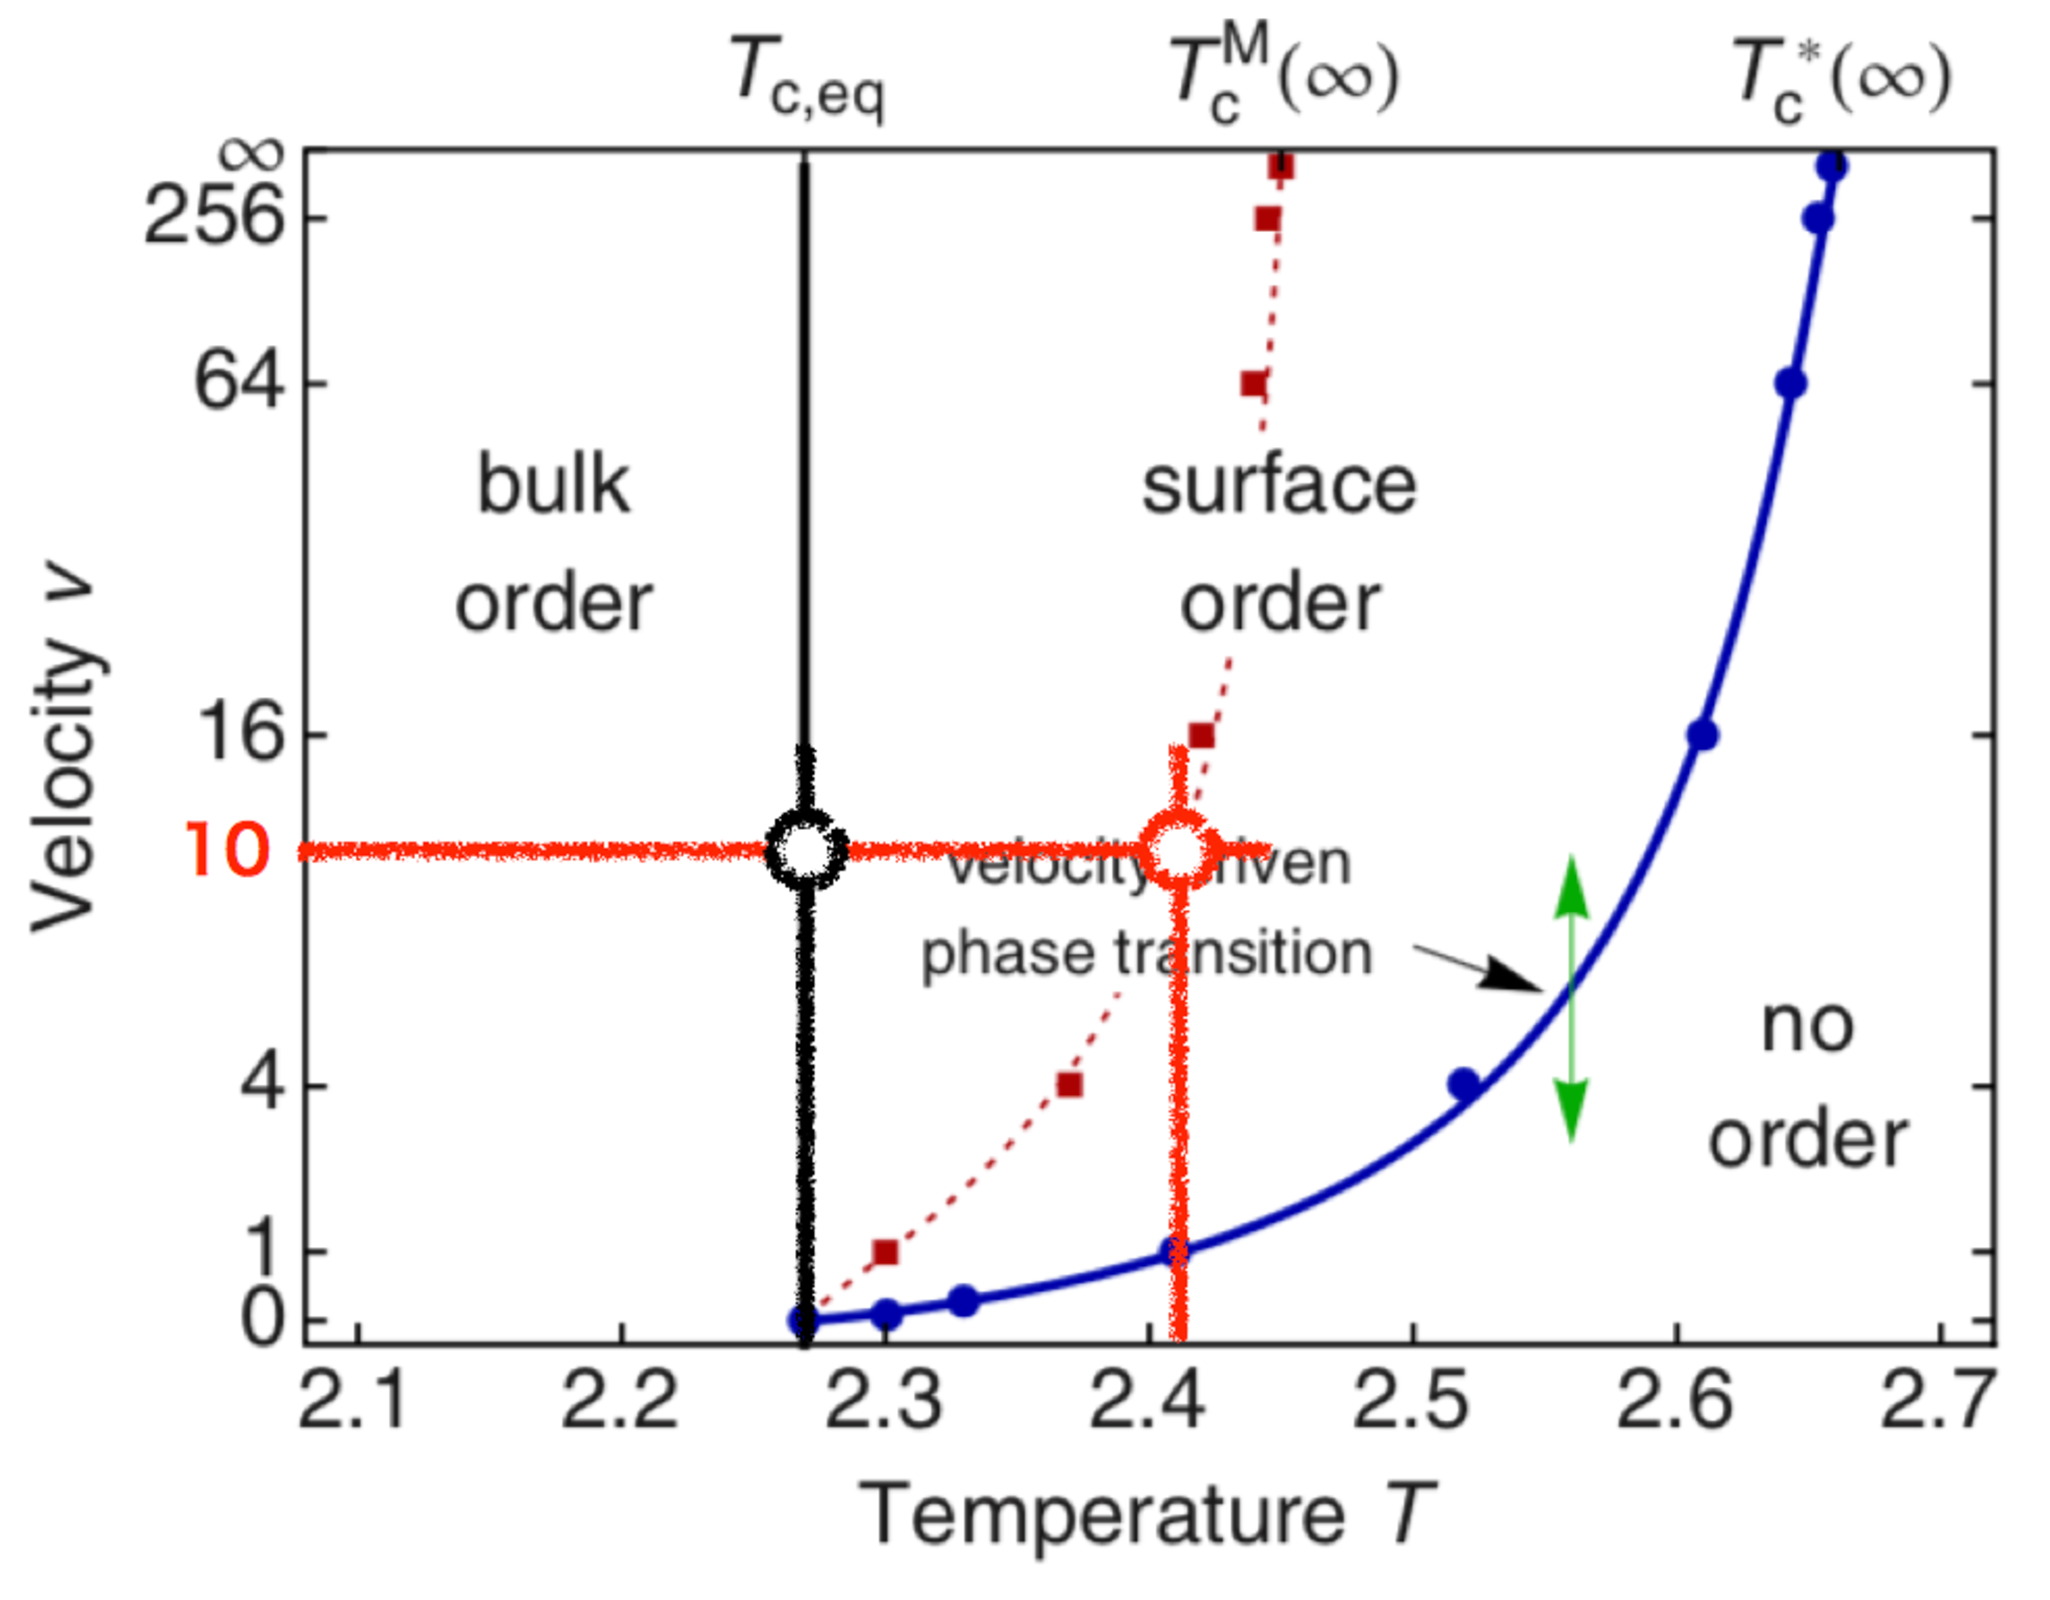
\includegraphics[width=0.5\linewidth]{NEPTIsing_.pdf}
	\caption{The non-equilibrium critical temperature $T^{\rm M}_{\rm c}(v)\simeq 2.40$ (the vertical red line) with the velocity $v\simeq 10$ and the equilibrium critical temperature $T_{\rm c, eq}\simeq 2.27$ (the vertical black line) in the phase diagram of the two-dimensional non-equilibrium Ising model obtained in Ref.~\cite{Hucht2009b}\protect\footnotemark.}
	\label{fig:NEPTinIsing_}
\end{figure}

\footnotetext{Reprinted Fig.~15 with permission from \fullcite{Hucht2009b}. Copyright (2018) by the American Physical Society.}

We also consider the reason why not only the heat capacity $c(L_{z}, T)$ but also the temperature derivative of the frictional force density $\partial f(L_{z}, T)/\partial T$ shows the divergent behavior. The frictional force density $f(L_{z}, T)$ is estimated by the difference between the expectation value of the energy before and after the sliding. It is therefore plausible that both expectation values have a singularity near $k_{\rm B}T/J=2.40$, and these singularities do not cancel with each other.

\section{Checking the Convergence in the Limit $L_{x}\to\infty$}
\label{sec:convcheck}

We now demonstrate that the following two observables converge in the infinite-size limit $L_{x}\to\infty$:

\begin{align}
f(L_{z}, T):=&\lim_{L_{x}\to\infty}\frac{F(L_{x}, L_{z}, T)}{L_{x}},\\
\epsilon(L_{z}, T):=&\lim_{L_{x}\to\infty}\frac{E_{b}(L_{x}. L_{z}, T)}{L_{x}L_{z}}.
\end{align}
We use the aspect ratios of $L_{x}=30\times L_{z}, 40\times L_{z}, 50\times L_{z}$ with $L_{z}$ fixed in order to check the convergence in the limit $L_{x}/L_{z}\to\infty$. Figures~\ref{fig:ffdcheck1}, \ref{fig:ffdcheck2}, \ref{fig:ebcheck1} and \ref{fig:ebcheck2} respectively show the temperature dependence of the frictional force density and the energy density under each set of boundary conditions for each size of $L_{z} = 4, 8, 16, 32, 64$. We see the quantities $F(L_{x}, L_{z}, T)/L_{x}$ and $E(L_{x}, L_{z}, T)/L_{x}$ for each set of boundary conditions have little dependence on $L_{x}$ for sufficiently large size of $L_{x}$ with each size of $L_{z}$.

\begin{figure}[htbp]
	\centering
	\subcaptionbox{\label{fig:ffdcheckfor004}}[0.80\linewidth]{\includegraphics[width=0.55\linewidth]{../../NumCalc/ClassicalSpinMC/FricDensP_Lz004.eps}}
	
	\subcaptionbox{\label{fig:ffdcheckfor008}}[0.80\linewidth]{\includegraphics[width=0.55\linewidth]{../../NumCalc/ClassicalSpinMC/FricDensP_Lz008.eps}}
	
	\subcaptionbox{\label{fig:ffdcheckfor016}}[0.80\linewidth]{\includegraphics[width=0.55\linewidth]{../../NumCalc/ClassicalSpinMC/FricDensP_Lz016.eps}}
	
	\caption{Each panel shows $F(L_{x}, L_{z}, T)/L_{x}$ against the temperature $T$: (\subref{fig:ffdcheckfor004}) $L_{z}=4$; (\subref{fig:ffdcheckfor008}) $L_{z}=8$; (\subref{fig:ffdcheckfor016}) $L_{z}=16$.}
	\label{fig:ffdcheck1}
\end{figure}

\begin{figure}[htbp]
	\centering
	\subcaptionbox{\label{fig:ffdcheckfor032}}[0.80\linewidth]{\includegraphics[width=0.55\linewidth]{../../NumCalc/ClassicalSpinMC/FricDensP_Lz032.eps}}
	
	\subcaptionbox{\label{fig:ffdcheckfor064}}[0.80\linewidth]{\includegraphics[width=0.55\linewidth]{../../NumCalc/ClassicalSpinMC/FricDensP_Lz064.eps}}
	
	\caption{Each panel shows $F(L_{x}, L_{z}, T)/L_{x}$ against the temperature $T$: (\subref{fig:ffdcheckfor032}) $L_{z}=32$; (\subref{fig:ffdcheckfor064}) $L_{z}=64$.}
	\label{fig:ffdcheck2}
\end{figure}

\begin{figure}[htbp]
	\centering
	\subcaptionbox{\label{fig:ebcheckfor004}}[0.80\linewidth]{\includegraphics[width=0.55\linewidth]{../../NumCalc/ClassicalSpinMC/EnDens_Lz004.eps}}
	
	\subcaptionbox{\label{fig:ebcheckfor008}}[0.80\linewidth]{\includegraphics[width=0.55\linewidth]{../../NumCalc/ClassicalSpinMC/EnDens_Lz008.eps}}
	
	\subcaptionbox{\label{fig:ebcheckfor016}}[0.80\linewidth]{\includegraphics[width=0.55\linewidth]{../../NumCalc/ClassicalSpinMC/EnDens_Lz016.eps}}
	
	\caption{Each panel shows $E(L_{x}, L_{z}, T)/(L_{x}L_{z})$ against the temperature $T$: (\subref{fig:ffdcheckfor004}) $L_{z}=4$; (\subref{fig:ffdcheckfor008}) $L_{z}=8$; (\subref{fig:ffdcheckfor016}) $L_{z}=16$.}
	\label{fig:ebcheck1}
\end{figure}

\begin{figure}[htbp]
	\centering
	\subcaptionbox{\label{fig:ebcheckfor032}}[0.80\linewidth]{\includegraphics[width=0.55\linewidth]{../../NumCalc/ClassicalSpinMC/EnDens_Lz032.eps}}
	
	\subcaptionbox{\label{fig:ebcheckfor064}}[0.80\linewidth]{\includegraphics[width=0.55\linewidth]{../../NumCalc/ClassicalSpinMC/EnDens_Lz064.eps}}
	
	\caption{Each panel shows $E(L_{x}, L_{z}, T)/(L_{x}L_{z})$ against the temperature $T$: (\subref{fig:ffdcheckfor032}) $L_{z}=32$; (\subref{fig:ffdcheckfor064}) $L_{z}=64$.}
	\label{fig:ebcheck2}
\end{figure}

%\section{Time Series of Observables}\label{appsec:timeconvcheck}
%
%\renewcommand\thefigure{\thesection.\arabic{figure}}
%\renewcommand\thesubfigure{\thefigure.\arabic{subfigure}}
%
%We now show the data which we use to calculate the long time limit of power  $P(t)$, dissipation rate $D(t)$ and bulk energy $E_{\rm b}(t)$.
%
%We can estimate the non-equilibrium correlation time of these observables, and then the valid interval in each time series are determined.
%
%\subsection{Bulk Energy Densities for the Anti-parallel Boundary Condition}
%
%\subsubsection{With the Size of $L_{z}=4$, $L_{x}=40$}
%\begin{figure}[htbp]
%	\centering
%	\subcaptionbox{$k_{\rm B}T/J=5.0$}{\includegraphics[width=0.3\linewidth]{../../NumCalc/ClassicalSpinMC/dat/Lz004Lx0040Ly__Vel10/antiparallel/ed_beta.200.eps}}
%	\subcaptionbox{$k_{\rm B}T/J=4.9$}{\includegraphics[width=0.3\linewidth]{../../NumCalc/ClassicalSpinMC/dat/Lz004Lx0040Ly__Vel10/antiparallel/ed_beta.204.eps}}
%	\subcaptionbox{$k_{\rm B}T/J=4.8$}{\includegraphics[width=0.3\linewidth]{../../NumCalc/ClassicalSpinMC/dat/Lz004Lx0040Ly__Vel10/antiparallel/ed_beta.208.eps}}
%
%	\subcaptionbox{$k_{\rm B}T/J=4.7$}{\includegraphics[width=0.3\linewidth]{../../NumCalc/ClassicalSpinMC/dat/Lz004Lx0040Ly__Vel10/antiparallel/ed_beta.212.eps}}
%	\subcaptionbox{$k_{\rm B}T/J=4.6$}{\includegraphics[width=0.3\linewidth]{../../NumCalc/ClassicalSpinMC/dat/Lz004Lx0040Ly__Vel10/antiparallel/ed_beta.217.eps}}
%	\subcaptionbox{$k_{\rm B}T/J=4.5$}{\includegraphics[width=0.3\linewidth]{../../NumCalc/ClassicalSpinMC/dat/Lz004Lx0040Ly__Vel10/antiparallel/ed_beta.222.eps}}
%
%	\subcaptionbox{$k_{\rm B}T/J=4.4$}{\includegraphics[width=0.3\linewidth]{../../NumCalc/ClassicalSpinMC/dat/Lz004Lx0040Ly__Vel10/antiparallel/ed_beta.227.eps}}
%	\subcaptionbox{$k_{\rm B}T/J=4.3$}{\includegraphics[width=0.3\linewidth]{../../NumCalc/ClassicalSpinMC/dat/Lz004Lx0040Ly__Vel10/antiparallel/ed_beta.232.eps}}
%	\subcaptionbox{$k_{\rm B}T/J=4.2$}{\includegraphics[width=0.3\linewidth]{../../NumCalc/ClassicalSpinMC/dat/Lz004Lx0040Ly__Vel10/antiparallel/ed_beta.238.eps}}
%
%	\subcaptionbox{$k_{\rm B}T/J=4.1$}{\includegraphics[width=0.3\linewidth]{../../NumCalc/ClassicalSpinMC/dat/Lz004Lx0040Ly__Vel10/antiparallel/ed_beta.243.eps}}
%	\subcaptionbox{$k_{\rm B}T/J=4.0$}{\includegraphics[width=0.3\linewidth]{../../NumCalc/ClassicalSpinMC/dat/Lz004Lx0040Ly__Vel10/antiparallel/ed_beta.250.eps}}
%	\subcaptionbox{$k_{\rm B}T/J=3.9$}{\includegraphics[width=0.3\linewidth]{../../NumCalc/ClassicalSpinMC/dat/Lz004Lx0040Ly__Vel10/antiparallel/ed_beta.256.eps}}
%
%	\subcaptionbox{$k_{\rm B}T/J=3.8$}{\includegraphics[width=0.3\linewidth]{../../NumCalc/ClassicalSpinMC/dat/Lz004Lx0040Ly__Vel10/antiparallel/ed_beta.263.eps}}
%	\subcaptionbox{$k_{\rm B}T/J=3.7$}{\includegraphics[width=0.3\linewidth]{../../NumCalc/ClassicalSpinMC/dat/Lz004Lx0040Ly__Vel10/antiparallel/ed_beta.270.eps}}
%	\subcaptionbox{$k_{\rm B}T/J=3.6$}{\includegraphics[width=0.3\linewidth]{../../NumCalc/ClassicalSpinMC/dat/Lz004Lx0040Ly__Vel10/antiparallel/ed_beta.277.eps}}
%	
%	\caption{Each data shows $\epsilon_{\rm b}(L_{x}, L_{z}, T)/(L_{x}L_{z})$ versus $t$.}
%\end{figure}
%
%\begin{figure}[htbp]
%	\centering
%	\subcaptionbox{$k_{\rm B}T/J=3.5$}{\includegraphics[width=0.3\linewidth]{../../NumCalc/ClassicalSpinMC/dat/Lz004Lx0040Ly__Vel10/antiparallel/ed_beta.285.eps}}
%	\subcaptionbox{$k_{\rm B}T/J=3.4$}{\includegraphics[width=0.3\linewidth]{../../NumCalc/ClassicalSpinMC/dat/Lz004Lx0040Ly__Vel10/antiparallel/ed_beta.294.eps}}
%	\subcaptionbox{$k_{\rm B}T/J=3.3$}{\includegraphics[width=0.3\linewidth]{../../NumCalc/ClassicalSpinMC/dat/Lz004Lx0040Ly__Vel10/antiparallel/ed_beta.303.eps}}
%
%	\subcaptionbox{$k_{\rm B}T/J=3.2$}{\includegraphics[width=0.3\linewidth]{../../NumCalc/ClassicalSpinMC/dat/Lz004Lx0040Ly__Vel10/antiparallel/ed_beta.312.eps}}
%	\subcaptionbox{$k_{\rm B}T/J=3.1$}{\includegraphics[width=0.3\linewidth]{../../NumCalc/ClassicalSpinMC/dat/Lz004Lx0040Ly__Vel10/antiparallel/ed_beta.322.eps}}
%	\subcaptionbox{$k_{\rm B}T/J=3.0$}{\includegraphics[width=0.3\linewidth]{../../NumCalc/ClassicalSpinMC/dat/Lz004Lx0040Ly__Vel10/antiparallel/ed_beta.333.eps}}
%
%	\subcaptionbox{$k_{\rm B}T/J=2.9$}{\includegraphics[width=0.3\linewidth]{../../NumCalc/ClassicalSpinMC/dat/Lz004Lx0040Ly__Vel10/antiparallel/ed_beta.344.eps}}
%	\subcaptionbox{$k_{\rm B}T/J=2.8$}{\includegraphics[width=0.3\linewidth]{../../NumCalc/ClassicalSpinMC/dat/Lz004Lx0040Ly__Vel10/antiparallel/ed_beta.357.eps}}
%	\subcaptionbox{$k_{\rm B}T/J=2.7$}{\includegraphics[width=0.3\linewidth]{../../NumCalc/ClassicalSpinMC/dat/Lz004Lx0040Ly__Vel10/antiparallel/ed_beta.370.eps}}
%
%	\subcaptionbox{$k_{\rm B}T/J=2.6$}{\includegraphics[width=0.3\linewidth]{../../NumCalc/ClassicalSpinMC/dat/Lz004Lx0040Ly__Vel10/antiparallel/ed_beta.384.eps}}
%	\subcaptionbox{$k_{\rm B}T/J=2.50$}{\includegraphics[width=0.3\linewidth]{../../NumCalc/ClassicalSpinMC/dat/Lz004Lx0040Ly__Vel10/antiparallel/ed_beta.400.eps}}
%	\subcaptionbox{$k_{\rm B}T/J=2.48$}{\includegraphics[width=0.3\linewidth]{../../NumCalc/ClassicalSpinMC/dat/Lz004Lx0040Ly__Vel10/antiparallel/ed_beta.403.eps}}
%
%	\subcaptionbox{$k_{\rm B}T/J=2.46$}{\includegraphics[width=0.3\linewidth]{../../NumCalc/ClassicalSpinMC/dat/Lz004Lx0040Ly__Vel10/antiparallel/ed_beta.406.eps}}
%	\subcaptionbox{$k_{\rm B}T/J=2.44$}{\includegraphics[width=0.3\linewidth]{../../NumCalc/ClassicalSpinMC/dat/Lz004Lx0040Ly__Vel10/antiparallel/ed_beta.409.eps}}
%	\subcaptionbox{$k_{\rm B}T/J=2.42$}{\includegraphics[width=0.3\linewidth]{../../NumCalc/ClassicalSpinMC/dat/Lz004Lx0040Ly__Vel10/antiparallel/ed_beta.413.eps}}
%	
%	\caption{Each data shows $\epsilon_{\rm b}(L_{x}, L_{z}, T)/(L_{x}L_{z})$ versus $t$.}
%\end{figure}
%
%\begin{figure}[htbp]
%	\centering
%	\subcaptionbox{$k_{\rm B}T/J=2.40$}{\includegraphics[width=0.3\linewidth]{../../NumCalc/ClassicalSpinMC/dat/Lz004Lx0040Ly__Vel10/antiparallel/ed_beta.416.eps}}
%	\subcaptionbox{$k_{\rm B}T/J=2.38$}{\includegraphics[width=0.3\linewidth]{../../NumCalc/ClassicalSpinMC/dat/Lz004Lx0040Ly__Vel10/antiparallel/ed_beta.420.eps}}
%	\subcaptionbox{$k_{\rm B}T/J=2.36$}{\includegraphics[width=0.3\linewidth]{../../NumCalc/ClassicalSpinMC/dat/Lz004Lx0040Ly__Vel10/antiparallel/ed_beta.423.eps}}
%
%	\subcaptionbox{$k_{\rm B}T/J=2.34$}{\includegraphics[width=0.3\linewidth]{../../NumCalc/ClassicalSpinMC/dat/Lz004Lx0040Ly__Vel10/antiparallel/ed_beta.427.eps}}
%	\subcaptionbox{$k_{\rm B}T/J=2.32$}{\includegraphics[width=0.3\linewidth]{../../NumCalc/ClassicalSpinMC/dat/Lz004Lx0040Ly__Vel10/antiparallel/ed_beta.431.eps}}
%	\subcaptionbox{$k_{\rm B}T/J=2.30$}{\includegraphics[width=0.3\linewidth]{../../NumCalc/ClassicalSpinMC/dat/Lz004Lx0040Ly__Vel10/antiparallel/ed_beta.434.eps}}
%
%	\subcaptionbox{$k_{\rm B}T/J=2.26$}{\includegraphics[width=0.3\linewidth]{../../NumCalc/ClassicalSpinMC/dat/Lz004Lx0040Ly__Vel10/antiparallel/ed_beta.442.eps}}
%	\subcaptionbox{$k_{\rm B}T/J=2.24$}{\includegraphics[width=0.3\linewidth]{../../NumCalc/ClassicalSpinMC/dat/Lz004Lx0040Ly__Vel10/antiparallel/ed_beta.446.eps}}
%	\subcaptionbox{$k_{\rm B}T/J=2.22$}{\includegraphics[width=0.3\linewidth]{../../NumCalc/ClassicalSpinMC/dat/Lz004Lx0040Ly__Vel10/antiparallel/ed_beta.450.eps}}
%
%	\subcaptionbox{$k_{\rm B}T/J=2.20$}{\includegraphics[width=0.3\linewidth]{../../NumCalc/ClassicalSpinMC/dat/Lz004Lx0040Ly__Vel10/antiparallel/ed_beta.454.eps}}
%	\subcaptionbox{$k_{\rm B}T/J=2.18$}{\includegraphics[width=0.3\linewidth]{../../NumCalc/ClassicalSpinMC/dat/Lz004Lx0040Ly__Vel10/antiparallel/ed_beta.458.eps}}
%	\subcaptionbox{$k_{\rm B}T/J=2.16$}{\includegraphics[width=0.3\linewidth]{../../NumCalc/ClassicalSpinMC/dat/Lz004Lx0040Ly__Vel10/antiparallel/ed_beta.462.eps}}
%
%	\subcaptionbox{$k_{\rm B}T/J=2.14$}{\includegraphics[width=0.3\linewidth]{../../NumCalc/ClassicalSpinMC/dat/Lz004Lx0040Ly__Vel10/antiparallel/ed_beta.467.eps}}
%	\subcaptionbox{$k_{\rm B}T/J=2.12$}{\includegraphics[width=0.3\linewidth]{../../NumCalc/ClassicalSpinMC/dat/Lz004Lx0040Ly__Vel10/antiparallel/ed_beta.471.eps}}
%	\subcaptionbox{$k_{\rm B}T/J=2.10$}{\includegraphics[width=0.3\linewidth]{../../NumCalc/ClassicalSpinMC/dat/Lz004Lx0040Ly__Vel10/antiparallel/ed_beta.476.eps}}
%	\caption{Each data shows $\epsilon_{\rm b}(L_{x}, L_{z}, T)/(L_{x}L_{z})$ versus $t$.}
%\end{figure}
%
%\begin{figure}[htbp]
%	\centering
%	\subcaptionbox{$k_{\rm B}T/J=2.08$}{\includegraphics[width=0.3\linewidth]{../../NumCalc/ClassicalSpinMC/dat/Lz004Lx0040Ly__Vel10/antiparallel/ed_beta.480.eps}}
%	\subcaptionbox{$k_{\rm B}T/J=2.06$}{\includegraphics[width=0.3\linewidth]{../../NumCalc/ClassicalSpinMC/dat/Lz004Lx0040Ly__Vel10/antiparallel/ed_beta.485.eps}}
%	\subcaptionbox{$k_{\rm B}T/J=2.04$}{\includegraphics[width=0.3\linewidth]{../../NumCalc/ClassicalSpinMC/dat/Lz004Lx0040Ly__Vel10/antiparallel/ed_beta.490.eps}}
%
%	\subcaptionbox{$k_{\rm B}T/J=2.02$}{\includegraphics[width=0.3\linewidth]{../../NumCalc/ClassicalSpinMC/dat/Lz004Lx0040Ly__Vel10/antiparallel/ed_beta.495.eps}}
%	\subcaptionbox{$k_{\rm B}T/J=1.9$}{\includegraphics[width=0.3\linewidth]{../../NumCalc/ClassicalSpinMC/dat/Lz004Lx0040Ly__Vel10/antiparallel/ed_beta.526.eps}}
%	\subcaptionbox{$k_{\rm B}T/J=1.8$}{\includegraphics[width=0.3\linewidth]{../../NumCalc/ClassicalSpinMC/dat/Lz004Lx0040Ly__Vel10/antiparallel/ed_beta.555.eps}}
%
%	\subcaptionbox{$k_{\rm B}T/J=1.7$}{\includegraphics[width=0.3\linewidth]{../../NumCalc/ClassicalSpinMC/dat/Lz004Lx0040Ly__Vel10/antiparallel/ed_beta.588.eps}}
%	\subcaptionbox{$k_{\rm B}T/J=1.6$}{\includegraphics[width=0.3\linewidth]{../../NumCalc/ClassicalSpinMC/dat/Lz004Lx0040Ly__Vel10/antiparallel/ed_beta.625.eps}}
%	\subcaptionbox{$k_{\rm B}T/J=1.5$}{\includegraphics[width=0.3\linewidth]{../../NumCalc/ClassicalSpinMC/dat/Lz004Lx0040Ly__Vel10/antiparallel/ed_beta.666.eps}}
%
%	\subcaptionbox{$k_{\rm B}T/J=1.4$}{\includegraphics[width=0.3\linewidth]{../../NumCalc/ClassicalSpinMC/dat/Lz004Lx0040Ly__Vel10/antiparallel/ed_beta.714.eps}}
%	\subcaptionbox{$k_{\rm B}T/J=1.3$}{\includegraphics[width=0.3\linewidth]{../../NumCalc/ClassicalSpinMC/dat/Lz004Lx0040Ly__Vel10/antiparallel/ed_beta.769.eps}}
%	\subcaptionbox{$k_{\rm B}T/J=1.2$}{\includegraphics[width=0.3\linewidth]{../../NumCalc/ClassicalSpinMC/dat/Lz004Lx0040Ly__Vel10/antiparallel/ed_beta.833.eps}}
%
%	\subcaptionbox{$k_{\rm B}T/J=1.1$}{\includegraphics[width=0.3\linewidth]{../../NumCalc/ClassicalSpinMC/dat/Lz004Lx0040Ly__Vel10/antiparallel/ed_beta.909.eps}}
%	\subcaptionbox{$k_{\rm B}T/J=1.0$}{\includegraphics[width=0.3\linewidth]{../../NumCalc/ClassicalSpinMC/dat/Lz004Lx0040Ly__Vel10/antiparallel/ed_beta1.000.eps}}
%	\subcaptionbox{$k_{\rm B}T/J=0.9$}{\includegraphics[width=0.3\linewidth]{../../NumCalc/ClassicalSpinMC/dat/Lz004Lx0040Ly__Vel10/antiparallel/ed_beta1.111.eps}}
%	\caption{Each data shows $\epsilon_{\rm b}(L_{x}, L_{z}, T)/(L_{x}L_{z})$ versus $t$.}
%\end{figure}
%
%\begin{figure}[htbp]
%	\centering
%	\subcaptionbox{$k_{\rm B}T/J=0.8$}{\includegraphics[width=0.3\linewidth]{../../NumCalc/ClassicalSpinMC/dat/Lz004Lx0040Ly__Vel10/antiparallel/ed_beta1.250.eps}}
%	\subcaptionbox{$k_{\rm B}T/J=0.7$}{\includegraphics[width=0.3\linewidth]{../../NumCalc/ClassicalSpinMC/dat/Lz004Lx0040Ly__Vel10/antiparallel/ed_beta1.428.eps}}
%	\subcaptionbox{$k_{\rm B}T/J=0.6$}{\includegraphics[width=0.3\linewidth]{../../NumCalc/ClassicalSpinMC/dat/Lz004Lx0040Ly__Vel10/antiparallel/ed_beta1.666.eps}}
%
%	\subcaptionbox{$k_{\rm B}T/J=0.5$}{\includegraphics[width=0.3\linewidth]{../../NumCalc/ClassicalSpinMC/dat/Lz004Lx0040Ly__Vel10/antiparallel/ed_beta2.000.eps}}
%	\subcaptionbox{$k_{\rm B}T/J=0.4$}{\includegraphics[width=0.3\linewidth]{../../NumCalc/ClassicalSpinMC/dat/Lz004Lx0040Ly__Vel10/antiparallel/ed_beta2.500.eps}}
%	\subcaptionbox{$k_{\rm B}T/J=0.3$}{\includegraphics[width=0.3\linewidth]{../../NumCalc/ClassicalSpinMC/dat/Lz004Lx0040Ly__Vel10/antiparallel/ed_beta3.333.eps}}
%
%	\subcaptionbox{$k_{\rm B}T/J=0.2$}{\includegraphics[width=0.3\linewidth]{../../NumCalc/ClassicalSpinMC/dat/Lz004Lx0040Ly__Vel10/antiparallel/ed_beta5.000.eps}}
%	\subcaptionbox{$k_{\rm B}T/J=0.1$}{\includegraphics[width=0.3\linewidth]{../../NumCalc/ClassicalSpinMC/dat/Lz004Lx0040Ly__Vel10/antiparallel/ed_beta10.000.eps}}
%	\caption{Each data shows $\epsilon_{\rm b}(L_{x}, L_{z}, T)/(L_{x}L_{z})$ versus $t$.}
%\end{figure}
%
%\subsubsection{With the Size of $L_{z}=4$, $L_{x}=80$}
%
%\subsubsection{With the Size of $L_{z}=4$, $L_{x}=120$}
%
%\subsubsection{With the Size of $L_{z}=4$, $L_{x}=160$}
%
%\subsubsection{With the Size of $L_{z}=4$, $L_{x}=300$}
%
%\subsection{Bulk Energy Densities for the Parallel Boundary Condition}
